% Use only LaTeX2e, calling the article.cls class and 12-point type.

\documentclass[12pt]{article}

% Users of the {thebibliography} environment or BibTeX should use the
% scicite.sty package, downloadable from *Science* at
% www.sciencemag.org/about/authors/prep/TeX_help/ .
% This package should properly format in-text
% reference calls and reference-list numbers.

\usepackage{scicite}

% Use times if you have the font installed; otherwise, comment out the
% following line.

\usepackage{times}

\usepackage{enumitem}
\usepackage{float}
\usepackage{graphicx}

% The preamble here sets up a lot of new/revised commands and
% environments.  It's annoying, but please do *not* try to strip these
% out into a separate .sty file (which could lead to the loss of some
% information when we convert the file to other formats).  Instead, keep
% them in the preamble of your main LaTeX source file.


% The following parameters seem to provide a reasonable page setup.

\topmargin 0.0cm
\oddsidemargin 0.2cm
\textwidth 16cm 
\textheight 21cm
\footskip 1.0cm


%The next command sets up an environment for the abstract to your paper.

\newenvironment{sciabstract}{%
\begin{quote} \bf}
{\end{quote}}


% If your reference list includes text notes as well as references,
% include the following line; otherwise, comment it out.

\renewcommand\refname{References and Notes}

% The following lines set up an environment for the last note in the
% reference list, which commonly includes acknowledgments of funding,
% help, etc.  It's intended for users of BibTeX or the {thebibliography}
% environment.  Users who are hand-coding their references at the end
% using a list environment such as {enumerate} can simply add another
% item at the end, and it will be numbered automatically.

\newcounter{lastnote}
\newenvironment{scilastnote}{%
\setcounter{lastnote}{\value{enumiv}}%
\addtocounter{lastnote}{+1}%
\begin{list}%
{\arabic{lastnote}.}
{\setlength{\leftmargin}{.22in}}
{\setlength{\labelsep}{.5em}}}
{\end{list}}


% Include your paper's title here

\title{Réduction Des Couches Convolutives Dans Les Réseaux Profonds} 


% Place the author information here.  Please hand-code the contact
% information and notecalls; do *not* use \footnote commands.  Let the
% author contact information appear immediately below the author names
% as shown.  We would also prefer that you don't change the type-size
% settings shown here.

\author
{Vincent Martineau,$^{1\ast}$\\
\\
\normalsize{$^{1}$Département d'informatique et de génie logiciel, Université Laval, Quebec, Canada}\\
\\
\normalsize{$^\ast$E-mail:  vincent.martineau.1@ulaval.ca.}
}

% Include the date command, but leave its argument blank.

\date{}



%%%%%%%%%%%%%%%%% END OF PREAMBLE %%%%%%%%%%%%%%%%



\begin{document} 

% Double-space the manuscript.

\baselineskip24pt

% Make the title.

\maketitle 



% Place your abstract within the special {sciabstract} environment.

\begin{sciabstract}
  Il y a eu des recherches expliquant comment réduire les couches de convolution dans les réseaux de neurones. Cependant dans les articles proposés les modèles utilisés sont généralement AlexNet et VGG. Lorsque ssayé sur des réseaux plus complexes tels que ResNet et DenseNet les solutions proposées ne fonctionnent pas. Le but ici est d'explorer les limites de cette approche et de proposer une solution afin de pouvoir généraliser à des réseaux plus complexes et profonds que ceux dans l'article original de Molchanov. Les expérimentations seront faites sur le transfert de modèle entre ImageNet vers Cifar10 et nous verrons les gains pouvant être faits sur des réseaux profonds. 
\end{sciabstract}



% In setting up this template for *Science* papers, we've used both
% the \section* command and the \paragraph* command for topical
% divisions.  Which you use will of course depend on the type of paper
% you're writing.  Review Articles tend to have displayed headings, for
% which \section* is more appropriate; Research Articles, when they have
% formal topical divisions at all, tend to signal them with bold text
% that runs into the paragraph, for which \paragraph* is the right
% choice.  Either way, use the asterisk (*) modifier, as shown, to
% suppress numbering.

\section*{Introduction}
Les réseaux CNN sont parmis nous depuis très longtemps\cite{lecunn1}. Ces réseaux sont très utilisés dans le traitement de l'image dans une grande variété de domaines. Ils sont très utilisé dans la classification ou la localisation d'objets. Que ce soit avec les systèmes de surveillance, les voitures automomes ou les appareils intelligents, ce type de réseaux fait maintenant partie de notre quotidien\cite{daily}.

Ces réseaux ont montré qu’ils pouvaient obtenir des résultats excédant les capacités humaines\cite{beathuman}. Dans plusieurs cas, ces modèles sont rendus disponibles au grand public et il est possible de les adapter à des problèmes plus simples pour obtenir de très bons résultats\cite{transfer}. 

\subsection{Description du problèmes}
Afin d'utiliser ces réseaux sûrs de petits appareils des techniques\cite{han1} ont été évalué dans le passé. Plus récemment, un article propose de faire la réduction de filtres de convolution\cite{molchanov}. Cependant l'article se concentre essentiellement sur les réseaux AlexNet et VGG et ne fonctionne pas sur les réseaux plus complexes présent dans PyTorch\cite{pytorchmodel}.

Le but de cet article sera d'évaluer le travail nécessaire pour pouvoir pousser cette logique vers des réseaux plus complexes tels que ResNet, DenseNet et SqueezeNet. 

\section*{Méthode}
La méthode utilisée est une variante de la méthode proposée dans l'article Pruning Convolutional Neural networks for Ressource efficient inference\cite{molchanov}. Le but des modifications est d'étendre les capacités de notre modèle à des réseaux beaucoup plus complexes tels que Res Net, DenseNet et Squeeze net. 

Voici une liste des étapes à suivre pour obtenir une réduction intéressante: 
\begin{enumerate}[noitemsep, noitemsep]
\item appliquer le fine tuning sur un réseau pré-entrainé. 
\item Extraire le graphe d'exécution de notre modèle 
\item à partir de notre graphe d'exécution, exclure les couches de convolution que nous ne voulons pas affecter. 
\item Réduire les filtres en fonction du critère de réduction 
\item Appliquer le fine tuning afin de restabiliser le réseau 
\item Recommencer la réduction tant que le réseau ne possède pas la taille voulue. 
\end{enumerate}

Dans cette procédure le critère de sélection est très important pour avoir de bons résultats. Pour cette expérimentation, nous avons utilisé les Taylor Expansions qui ont prouvé leur efficacité dans l'article et les activations moyennes. 

Afin de pouvoir exécuter sur des modèles plus complexes, nous avons choisi de ne pas explorer d'autres critères de sélection, mais bien de se concentrer sur l'algorithme nécessaire pour supporter des modèles plus complexes. 

\subsection{Les pratiques à éviter }
Dans la solution proposée, il est important de ne pas appliquer de réduction de filtres juste avant une addition de flow tel que vu dans plusieurs modèles complexes. La figure Figure1 représente cette situation. Le problème dans ce cas est qu’il est nécessaire d’appliquer une réduction équivalente sur toutes les branches entrantes.  Il est possible qu’il existe un critère de sélection permettant d’inclure ces couches dans le futur. 

\begin{figure}[H]
	\centering
	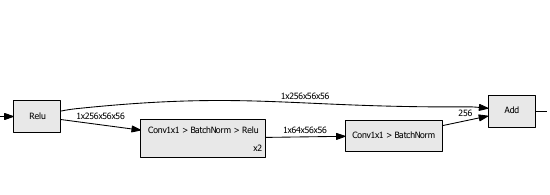
\includegraphics{residual_add}
	\caption{Description...}
	\label{fig:residualadd}
\end{figure}

Un autre problème potentiel survient lorsqu'une couche est réutilisée. Dans ce cas il faut que l'input de notre couche soit compatible avec la sortie de la couche que nous traitons. Cependant nous devons affecter les couches précédentes pour que les dimensions concordent aussi.

Il est à noter qu'il est possible qu'il existe un algorithme fiable qui permet de gérer ces cas, mais l'article présent n'explore pas ces options.

\subsection{Pratiques à éviter}
Lors de la construction du modèle il est très important d’éviter au maximum les valeurs fixes lors de l’inférence. Par exemple, dans le modèle AlexNet, il y a le code de la partie gauche de la figure 2 qui nous empêche de réduire la dernière couche de convolution avant la couche pleinement connectée. En effectuant la modification présenté dans la figure 2, il est maintenant possible de réduire la couche de convolution avant la couche pleinement connectée. 
\begin{figure}[H]
	\centering
	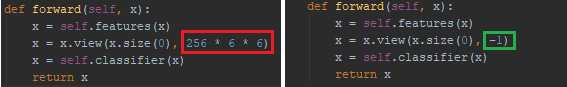
\includegraphics{mistake}
	\caption{Description...}
	\label{fig:mistake}
\end{figure}


\subsection{Propagation de l’effet}
Lorsqu’on retire un filtre de convolution d’une couche, il faut prendre plusieurs précautions pour assurer la stabilité du système. Par exemple, il faut ajuster les poids, le nombre de biais dans la couche et ajuster les gradients lorsque ces derniers sont contenus dans la couche elle-même. Ce qui est le cas de PyTorch.

Par la suite, il faut ajuster les couches suivantes en fonction de leur type.
Pour les couches de convolutions suivantes. Il est nécessaire d’ajuster le nombre de couches en entrées pour concorder avec la couche de convolution que nous traitons. Il faut aussi ajuster les poids de cette couche. 
Pour les couches de batch Norm, il faut ajuster les biais lorsqu'ils sont utilisés et nous effectuons un reset sur les variables utilisées à l’exécution. Dans PyTorch, nous parlons de running means et running vars. 
Finalement, nous devons ajuster les couches pleinement connectées. Dans le cas de ces couches, nous ajustons les poids et nous appliquons la weight inference rule\cite{weightinference} afin de simuler le retrait des poids par dropout. 
Les autres couches semblent bien supporter la réduction de couches de convolution. Il est à noter que nous avons uniquement essayé les modèles proposés dans PyTorch et que d'autres travail pourrait être nécessaire pour des couches plus complexes. 

\section*{Résultats}

\section*{Conclusion}

\bibliography{scibib}

\bibliographystyle{Science}


\end{document}




















